\title{An Introduction to the Objeck Programming Language}
\author{
        Randy Hollines \\
        objeck@gmail.com\\
}
\date{\today}

\documentclass[12pt]{article}

\usepackage{aliascnt}
\usepackage{hyperref}
\usepackage{MnSymbol}
\usepackage[pdftex]{graphicx}

\begin{document}

\maketitle
\thispagestyle{empty}

\vspace{\baselineskip}

\begin{abstract}
A brief introduction to the Objeck programming language and it's features.  This article is intended to introduce programmers and compiler designers to the unique features and design of the Objeck language.   Unless otherwise noted, this article covers functionality that is included in release \textit{0.9.10}.  For additional information please refer to the \htmladdnormallink{general}{http://sourceforge.net/projects/objeck-lang/} and \htmladdnormallink{technical}{http://code.google.com/p/objeck-lang/} project websites.
\end{abstract}

\newpage
\tableofcontents
\newpage

\label{Introduction}
\section{Introduction}
The Objeck program language is an object-oriented computer language that is designed to be a general purpose programming system.  The Objeck language allows programmers to quickly create solutions by leveraging pre-existing class libraries.  The syntax for the language was designed with symmetry in mind and enforces the notion that there should only be one way to do something. Features of this release include:
\begin{itemize}
	\item Support for object-oriented programming (all data types are treated as objects)
	\item Cross platform independence (OS X, Linux and Windows)
	\item Concurrent runtime JIT support for Intel processors
	\item Multi-threaded memory management (garbage collector)
	\item Basic block compiler optimizations
	\item Support for static libraries
	\item Interactive debugger
\end{itemize}

\section{Getting Started}

The Objeck computer language consist of a compiler and virtual machine.  The compiler program is named \texttt{obc}, while the runtime virtual machine (VM) program is named \texttt{obr}.  Here is the world famous ``Hello World" program written in the Objeck language:

\begin{verbatim}
bundle Default {
  class Hello {
    function : Main(args : String[]), Nil {
      "Hello World!"->PrintLine();
    }
  }
}
\end{verbatim}

\subsection{Compiling Source}
The example below compiles the source program \texttt{hello.obs} into the target binary file \texttt{hello.obe}.  The two output file types that the compilers supports are executables and shared libraries.  Shared libraries are binary files that contain all of the metadata needed by the compiler to relink them into programs.  Both executables and shared libraries contain enough metadata to support runtime introspection (a feature that will be added in a future release).  As a naming convention, executables must end in \texttt{*.obe} while shared libraries must end in \texttt{*.obl}.

Below is an example of compiling the ``Hello World" program
\begin{verbatim}
obc -src tests\hello.obs -dest hello.obe
\end{verbatim}

Additional compiler options are listed below:
\begin{center}
\begin{tabular}{| l | l |}
\hline
\emph{Option} & \emph{Description} \\ \hline \hline
\texttt{-src} & path to source files, delimited by the `\texttt{,}' character \\ \hline
\texttt{-lib} & path to library files, delimited by the `\texttt{,}' character \\ \hline
\texttt{-tar} & target output \texttt{exe} for executable and \texttt{lib} for library; default is  \texttt{exe} \\ \hline
\texttt{-opt} & optimization level \texttt{s0}--\texttt{s3} with \texttt{s3} being the most aggressive; default is \texttt{s0} \\ \hline
\texttt{-dest} & output file name \\ \hline
\texttt{-debug} & if set, produces debug out for use by the interactive debugger (see below) \\ \hline
\end{tabular}
\end{center}

\subsection{Executing}
The command line example below executes the \texttt{hello.obe} executable. Note, for executables all required libraries are statically linked in the target output file.  When compiling shared libraries, other shared libraries are \underline{not} linked into the target output library file.

\begin{verbatim}
obr hello.obe
\end{verbatim}

\section{The Basics}
Now lets introduce you the core features of the Objeck programming language.
\vspace{\baselineskip}

In Objeck, all data types are treated as objects. Basic objects provide supports for boolean, character, byte, integer and decimal types.  These basic objects can be used to create complex user defined objects.  The listing below defines the basic objects that are supported in the language:

\begin{center}
\begin{tabular}{| l | l |}
\hline
\emph{Type} & \emph{Description} \\ \hline \hline
\texttt{Char} &  1--byte character \\ \hline
\texttt{Char[]} &  character array \\ \hline
\texttt{Bool} &  boolean value \\ \hline
\texttt{Bool[]} &  boolean array \\ \hline
\texttt{Byte} &  1--byte integer \\ \hline
\texttt{Byte[]} &  byte array \\ \hline
\texttt{Int} &  4--byte integer \\ \hline
\texttt{Int[]} &  integer array \\ \hline
\texttt{Float} &  8--byte decimal \\ \hline
\texttt{Float[]} &  decimal array \\ \hline
\end{tabular}
\end{center}

As mentioned above, basic types are objects and have associated methods for each basic class type.  For example:

\begin{verbatim}
13->Min(3)->PrintLine();
13->Max(3)->PrintLine();
-22->Abs()->PrintLine();
Float->Pi()->PrintLine();
\end{verbatim}

\subsection{Variable Declarations}
Variables can be declared for all of the basic types described above and for user defined objects. Variables can be declared anywhere in a program and are bound to traditional block scoping rules.  Variable assignments can be made during a declaration or at any other point in a program. Variables may be declared as local, class instance or class variables.  Class level variables are declared using the \texttt{static} keyword. A class that is derived from another class may access it's parents variables if the parent class is declared in one of the source programs.  \textit{If a class is derived from a class declared in a shared library then that class cannot access it's parents variables, unless an accessor method is provided.}  Local variables can be declared without specifying their data type, such variables are bound to a type following their first assignment. Three different declaration styles are shown below:

\begin{verbatim}
a : Int;
b : Int := 13;
c := 7;
\end{verbatim}

Types that are not initialized at declaration time are initialized with the following default values:

\vspace{\baselineskip}
\begin{center}
\begin{tabular}{| l | c |}
\hline
\emph{Type} & \emph{Initialization} \\ \hline \hline
\texttt{Char} & `\textbackslash0' \\ \hline
\texttt{Byte} & 0 \\ \hline
\texttt{Int} & 0 \\ \hline
\texttt{Float} & 0.0 \\ \hline
Array & \texttt{Nil} \\ \hline
Object & \texttt{Nil} \\ \hline
\end{tabular}
\end{center}

\subsection{Expressions}
The Objeck language supports various expression types.  Some of these expression types include mathematical, logical, array and method call expressions.  The preceding sections describe some of the expressions that are supported in the Objeck language.

\subsubsection{Mathematical and Logical Expressions}
The following code example demonstrates two ways to printing the number \texttt{42}.  The first way invokes the \texttt{PrintLine()} method for the literal \texttt{42}.  The second prints the product of a variable and a literal.

\begin{verbatim}
bundle Default {
  class Test {
    function : Main(), Nil {
      42->PrintLine();
      eight := 8;
      (eight * 7)->PrintLine();
    }
  }
}
\end{verbatim}

The following mathematical operators are supported in the Objeck language for integers and decimal values:
\begin{itemize}
    \item addition (\texttt{+})
    \item subtraction (\texttt{-})
    \item multiplication (\texttt{*})
    \item division (\texttt{/})
    \item modulus -- (\texttt{\%} - for integer values only)
\end{itemize}

The [\texttt{*}, \texttt{/}, \texttt{\%}] operators have a higher precedence than  the [\texttt{+}, \texttt{-}] operators. Operators of the same precedence are evaluated from left-to-right.  Logical operations are of lower precedence than mathematical operations. All logical operators are of the same precedence and order is determined via left--to--right evaluation.  The [\texttt{\&}, \texttt{|}] logical operators use short-circuit logic; meaning that some expressions may not be executed if evaluation criteria is not satisfied.

The following logical operators are supported in the Objeck language:
\begin{itemize}
    \item and (\texttt{\&})
    \item or (\texttt{|})
    \item equal (\texttt{=})
    \item not--equal (\texttt{<>})
    \item less--than (\texttt{<})
    \item greater--than (\texttt{>})
    \item less--than--equal (\texttt{<=})
    \item greater--than--equal (\texttt{>=})
\end{itemize}

\subsubsection{Arrays}
The Objeck language supports single and multi-dimensional arrays.  Arrays are allocated dynamically from the system heap.  The memory that is allocated for arrays is managed automatically by the runtime garbage collector.  All of the basic types described above (as well as user defined types) can be allocated as arrays.  The code example below shows how a two-dimensional array of type \texttt{Int} is allocated and dereferenced.


\begin{verbatim}
array := Int->New[2,3];
array[0,2] := 13;
array[1,0] := 7;
\end{verbatim}

The size of an array can be obtained by calling the array's \texttt{GetSize()} method.  The \texttt{GetSize()} method will return the number of elements in a given array.  For a multi-dimensional array the size method returns the number of elements in the first dimension.  Character array literals are allocated as \texttt{String} objects.  It should also be noted that language has a \texttt{String} class that provides support for advanced string operations.

\begin{verbatim}
str := "Hello World!";
str->GetSize()->PrintLine();
\end{verbatim}

\subsection{Statements}
Besides providing support for declaration statements the language has support for conditional and control statements.  As with other languages, control statements can be nested in order to provide finer grain logical control. General control statements include \texttt{if} and \texttt{select} statements. Basic looping statements include \texttt{while}, \texttt{do/while} and \texttt{for} loops.  Note, all statements rather decelerations or controls end with a `\texttt{;}'.

\subsubsection{If Statement}

An \texttt{if} statement is a control statement that executes the associated block of code if it evaluates to \texttt{true}.  If the evaluation statement does not evaluate to \texttt{true} than an \texttt{else if} statement may be evaluated (if it exists), otherwise an \texttt{else} statement will be executed (if it exists).  The example below demonstrates an \texttt{if} statement.

\begin{verbatim}
value : Int := Console.ReadLine()->ToInt();
if(value <> 3) {
  "Not equal to 3"->PrintLine();
}
else if(value < 13) {
  "Less than 13"->PrintLine();
}
else {
  "Some other number"->PrintLine();
};
\end{verbatim}

\subsubsection{Select Statement}

A \texttt{select} statement maps a value to 1 or more labels.  Labels are associated to statement blocks.  A label may either be a literal or an \texttt{enum} value.  Multiple labels can be mapped to the same statement block.  Below is an example of a \texttt{select} statement.

\begin{verbatim}
select(v) {
   label Color->Red: {
      "Red"->PrintLine();
   }

   label 9:
   label 19: {
      v->PrintLine();
   }

   label 27: {
      (3 * 9)->PrintLine();
   }
};
\end{verbatim}

\subsubsection{While Statement}

A \texttt{while} statement is a control statement that will continue to execute its main body as long as its conditional expression evaluates to \texttt{true}.  When its conditional expression evaluates to \texttt{false} than the loop body will cease to execute.

\begin{verbatim}
i : Int := 10;
while(i > 0) {
   i->PrintLine();
   i := i - 1;
}
\end{verbatim}

\subsubsection{Do/While Statement}

A \texttt{do/while} statement is a control statement that will execute its main body at least once and continue to execute its main body as long as its conditional expression evaluates to \texttt{true}.  When its conditional expression evaluates to \texttt{false} than the loop body will cease to execute.

\begin{verbatim}
i : Int := 10;
do { 
   i->PrintLine();
   i := i - 1;
} 
while(i > 0);
\end{verbatim}

\subsubsection{For Statements}

The \texttt{for} statement is another common looping construct.  The \texttt{for} loop consists of a pre-condition statement followed by an evaluation expression and an update statement.

\begin{verbatim}
name : Char[] := "John"->ToCharArray();
for(i : Int := 0; i < name->GetSize(); i := i + 1;) {
  name[i]->PrintLine();
}
\end{verbatim}

\section{User Defined Types}

\subsection{Enums}
Enums are user defined enumerated types.  The main use of an  \texttt{enum}  is to group a class of countable values, for example colors, into a distinct class.  Once \texttt{enum}  values have been defined they may not be assigned or associated to a other \texttt{enum}  groups or integer classes.  The valid operations for enums are as follows:

\begin{itemize}
    \item assignment (\texttt{:=})
    \item equal (\texttt{=})
    \item not--equal (\texttt{<>})
\end{itemize}

In addition, enum values may be used in \texttt{select} statements as conditional tests or labels.

\begin{verbatim}
enum Color {
   Red,
   Black,
   Green
}
\end{verbatim}

\subsection{Classes}
Classes are user defined types that allow programmers to create specialized data types.  Classes are made up of attributes (data) and operations (methods).  Classes are used to encapsulate programming logic and localize information.  Operations that are associated to a class may either be at the class level or instance level.  Class instances are created by calling an object's \texttt{New()} function.  Note, an object instance can only be created if one or more \texttt{New()} functions have been defined.

\subsubsection{Class Inheritance}
Classes may be derived from other classes using the \texttt{from} keyword.  Class inheritance allows classes to share common functionality.  The Objeck language supports single class inheritance, meaning that a derived class may only have one parent.  The language also supports virtual classes, which assures that derived classes have been defined for all required operations declared in the base class.  Virtual classes also allow the programmer to define non-virtual methods that contain program behavior.  Virtual classes are dynamically bound to implementation classes at runtime.
\begin{verbatim}
class Foo {
  @lhs : Int;

  New(lhs : Int) {
    @lhs := lhs;
  }

  method : native : AddTwo(rhs : Int), Int {
    return 2 + rhs;
  }

  method : virtual : AddThree(int rhs), Int;

  method : GetLhs(), Int {
    return lhs;
  }
}

class Bar from Foo {
  New(value : Int) {
    Parent(value);
  }

  method : native : AddThree(rhs : Int), Int {
    return 3 + rhs;
  }

  function : Main(), Nil {
    bar : b := Bar->New(31);
    b->AddThree(9)->PrintLine();
  }
}
\end{verbatim}

\subsubsection{Class Casting and Identification}
An object that is inherited from another object may be either upcasted or downcasted.  Object casting can be performed using the \texttt{As()} operator.  The Object language detects upcasting and downcastng at compile time. Upcasting requires a runtime check, while down casting does not. If cross casting is detected then a compile time error will be generated.

\begin{verbatim}
method : public : Compare(right : Base), Int {
  if(right <> Nil) {
    if(GetClassID() = right->GetClassID()) {
      a : A := right->As(A);

      if(@value = a->GetValue()) {
        return 0;
      };
    ...	
\end{verbatim}

The class that a given object instance belongs to can found by calling its \texttt{GetClassID} method.  This method returns an enum that is associated with that instance's class type.  This method is generally used to determine if two object instances are of the same or different classes.

\subsubsection{Methods and Functions}
The Objeck language support both methods and functions.  Functions are public static procedures that may be executed by any class.  Methods are operations that may be performed on an object instance.  Methods have \texttt{public} and \texttt{private} qualifiers.  Methods that are \texttt{private} may only be called from within the same class, while \texttt{public} methods may be called from other classes.  Note, methods are \texttt{private} by default. The Objeck language supports polymorphic methods and functions, meaning that there can be multiple methods with the same name within the same class as long as their declaration arguments vary.

Methods and functions can either be executed in an interpreted or JIT compiled mode. Interpreted execution mimics microprocessor functions in a platform independent manner. JIT execution takes the compiled stack code an produces native machine code. Note, that there is initial overhead involved in the JIT compilation process since it occurs at runtime. In addition, some methods can not be compiled into native machine code but this is a rare case.  The keyword \texttt{native} is used to JIT compile methods and function at runtime.

A function or method may be defined as \texttt{virtual} meaning that any class that originates from that class must implement all of the class's \texttt{virtual} methods or functions.  \texttt{Virtual} methods are a way to ensure that certain operations are available to a family of classes. If a class declares a \texttt{virtual} method then the class become \texttt{virtual}, meaning that it cannot be directly instantiated.

Below is an example of declaring a virtual method:
\begin{verbatim}
method : virtual : public : Compare(right : Base), Int;
\end{verbatim}

\section{Interactive Debugger}
The Objeck compiler toolset contains a simple interactive read-only debugger, which allows programmers to inspect values within their programs.  The debugger allows programmers to set breakpoints within methods based upon source line numbers.  The debugger can also calculate simple arithmetic expressions involving variables and constants. The following commands are currently supported:

\begin{center}
\begin{tabular}{| l |p{4 cm} |p{6 cm} |}
\hline
\emph{Command} & \emph{Description} & \emph{Example} \\ \hline \hline
\texttt{[b]reak} &  sets a breakpoint & \texttt{b hello.obs:10} \\ \hline
\texttt{breaks} &  shows all breakpoints &  \\ \hline
\texttt{[d]elete} &  deletes a breakpoint & \texttt{d hello.obs:10} \\ \hline
\texttt{clear} &  clears all breakpoints &  \\ \hline
\texttt{[n]ext} &  moves to the next line with debug information &  \\ \hline
\texttt{[o]ut} &  jumps out of an existing method/function and moves to the next line with debug information &  \\ \hline
\texttt{args} &  specifies program arguments & \texttt{args "Hello World"} \\ \hline
\texttt{[r]un} &  runs a loaded program &  \\ \hline
\texttt{[p]rint} &  prints the value of an expression, along with metadata & \texttt{p @self$\rightarrow$value} \\ \hline
\texttt{[l]ist} &  lists a range of lines in a source file or the lines near the current breakpoint & \texttt{l hello.obs:10} \\ \hline
\texttt{[i]nfo} &  displays the variables for a class or method/function & \texttt{i class=Foo method=New} \\ \hline
\texttt{stack} &  displays the method/function call stack &  \\ \hline
\texttt{exe} &  loads a new executable & \texttt{exe "./../test.obe"} \\ \hline
\texttt{src} &  specifies a new source path & \texttt{src "../../"} \\ \hline
\texttt{[q]uit} &  exits a given debugging session &  \\ \hline
\end{tabular}
\end{center}

\subsection{Starting the Debugger}
The source program must be compiled with the \texttt{-debug} set. The command line debugger is started up running the \texttt{odb} executable. The \texttt{-exe} option must be present and specify the path to the executable.  The The \texttt{-src} option is optional and specifies the path to the program source.  Also note, to print instance level variables the path must start with \texttt{@self$\rightarrow$}. 

\subsection{Example Debugging Session}
\subsubsection{Sample Source}
\begin{verbatim}
bundle Default {
  class Bar {
    v1 : Float;
    v2 : Int;

    New() {
      v1 := 2.31;
      v2 := 26;
    }
  }

  class Foo {
    bar : Bar;
    value : Int;

    New(v : Int) {
      value := v;z
    }

    method : public : GetValue(), Int {
      return value;
    }

    method : public : SetBar(), Nil {
      bar := Bar->New();
    }
  }

  class Test {
    function : Main(args : System.String[]), Nil {
      d : Float := 11.12;
      z := Int->New[5,6];
      z[2,3] := 27;

      f := Foo->New(24);
      f->SetBar();
      v := f->GetValue();
    }
  }
}
\end{verbatim}
The sample file is named \texttt{debug.obs}.

\subsubsection{Compiling the Source and Starting the Debugger}
\begin{verbatim}
obc -src test_src\debug.obs -dest a.obe -debug
obd -exe ..\..\compiler\a.obe -src ..\..\compiler\test_src

-------------------------------------
Objeck v0.9.10 - Interactive Debugger
-------------------------------------
loaded executable: file='../../compiler/a.obe'
source files: path='../../compiler/test_src/'
\end{verbatim}

\subsubsection{Set a Breakpoint and Run Program}
\begin{verbatim}
> b debug.obs:31
added break point: file='debug.obs:31'
> r
break: file='debug.obs:31', method='Test->Main(..)'
> l
  List
     26: 		}
     27: 	}
     28: 
     29: 	class Test {
     30: 		function : Main(args : System.String[]), Nil {
=>   31: 			d : Float := 11.12;
     32: 			z := Int->New[5,6];	
     33: 			z[2,3] := 27;
     34: 
     35: 			f := Foo->New(24);
     36: 			f->SetBar();
> n
break: file='debug2.obs:32', method='Test->Main(..)'
\end{verbatim}

\subsubsection{Printing a Values}
\begin{verbatim}
> p d
print: type=Float, value=11.12
> b debug.obs:37
added break point: file='debug.obs:37'
> c
break: file='debug2.obs:37', method='Test->Main(..)'
> p z
print: type=Int[], value=2197556(0x218834), dimension=2, size=30
> p z[2,3]
print: type=Int[], value=27(0x1b)
>  p f->value
print: type=Int, value=24
> p f->bar
print: type=Bar, value=0x218864
> p f->bar->v1
print: type=Float, value=2.31
> q
> p f->bar->v1 * 3.5
print: type=Float, value=8.085
goodbye.
\end{verbatim}

\section{Class Libraries}
Objeck includes class libraries that provides access to system resources, such as files and sockets, while also providing support for  basic data structures like lists and vectors.  As new class libraries are added they will be documented in this section.

\subsection{Bool}
\begin{itemize}
    \item \texttt{Print} - prints the current value
    	\begin{itemize}
	\item method : native : Print(), Nil
	\end{itemize}
    \item \texttt{PrintLine} - prints the current value along with a line return
    	\begin{itemize}
	\item method : native : PrintLine(), Nil
	\end{itemize}
    \item \texttt{ToString} - converts the current value to a \texttt{String} object instance
   	\begin{itemize}
	\item method : native : ToString(), String
	\end{itemize}
\end{itemize}

\subsection{Char}
\begin{itemize}
    \item \texttt{IsDigit} - determines if the character is a digit (in the range of \texttt{0-9})
    	\begin{itemize}
	\item method : native : IsDigit(), Bool
	\end{itemize}
    \item \texttt{IsChar} - determines if the character is a alpha (in the range of \texttt{A-Z} or \texttt{a-z})
    	\begin{itemize}
	\item method : native : IsChar(), Bool
	\end{itemize}
    \item \texttt{Min} - returns the smallest of the two numbers; returns the same number if they are equal
    	\begin{itemize}
	\item method : native : Min(r : Byte), Byte
	\end{itemize}
    \item \texttt{Max} - returns the largest of the two numbers; returns the same number if they are equal
    	\begin{itemize}
	\item method : native : Max(r : Byte), Byte
	\end{itemize}
    \item \texttt{Print} - prints the current value
    	\begin{itemize}
	\item method : native : Print(), Nil
	\end{itemize}
    \item \texttt{PrintLine} - prints the current value along with a line return
    	\begin{itemize}
	\item method : native : PrintLine(), Nil
	\end{itemize}
    \item \texttt{ToString} - converts the current value to a \texttt{String} object instance
   	\begin{itemize}
	\item method : native : ToString(), String
	\end{itemize}
\end{itemize}

\subsection{Byte/Int}
\begin{itemize}
    \item \texttt{Min} - returns the smallest of the two numbers; returns the same number if they are equal
    	\begin{itemize}
	\item method : native : Min(r : Byte), Byte
	\end{itemize}
    \item \texttt{Max} - returns the largest of the two numbers; returns the same number if they are equal
    	\begin{itemize}
	\item method : native : Max(r : Byte), Byte
	\end{itemize}
    \item \texttt{Abs} - returns the absolute value of the current number
    	\begin{itemize}
	\item method : native : Abs(), Byte
	\end{itemize}
    \item \texttt{Print} - prints the current value
    	\begin{itemize}
	\item method : native : Print(), Nil
	\end{itemize}
    \item \texttt{PrintLine} - prints the current value along with a line return
    	\begin{itemize}
	\item method : native : PrintLine(), Nil
	\end{itemize}
    \item \texttt{ToString} - converts the current value to a \texttt{String} object instance
   	\begin{itemize}
	\item method : native : ToString(), String
	\end{itemize}
\end{itemize}

\subsection{Float}
\begin{itemize}
    \item \texttt{Min} - returns the smallest of the two numbers; returns the same number if they are equal
    	\begin{itemize}
	\item method : native : Min(r : Byte), Float
	\end{itemize}
    \item \texttt{Max} - returns the largest of the two numbers; returns the same number if they are equal
    	\begin{itemize}
	\item method : native : Max(r : Byte), Float
	\end{itemize}
    \item \texttt{Abs} - returns the absolute value of the current number
    	\begin{itemize}
	\item method : native : Abs(), Float
	\end{itemize}
    \item \texttt{Floor} - returns the floor of the current number
    	\begin{itemize}
	\item method : native : Floor(), Float
	\end{itemize}
    \item \texttt{Ceiling} - returns the ceiling of the current number
    	\begin{itemize}
	\item method : native : Ceiling(), Float
	\end{itemize}
    \item \texttt{Pi} - returns the value of Pi
    	\begin{itemize}
	\item function : native : Pi(), Float
	\end{itemize}
    \item \texttt{Print} - prints the current value
    	\begin{itemize}
	\item method : native : Print(), Nil
	\end{itemize}
    \item \texttt{PrintLine} - prints the current value along with a line return
    	\begin{itemize}
	\item method : native : PrintLine(), Nil
	\end{itemize}
    \item \texttt{ToString} - converts the current value to a \texttt{String} object instance
   	\begin{itemize}
	\item method : native : ToString(), String
	\end{itemize}
\end{itemize}

\subsection{String}
\begin{itemize}
    \item \texttt{New} 
    	\begin{itemize}
	\item New()
	\item New(s : String)
	\item New(a : Char[])
	\end{itemize}
    \item \texttt{Append} - Appends a \texttt{String}, \texttt{Char[]}, \texttt{Char}, \texttt{Int} or \texttt{Float} to the current String instance
    	\begin{itemize}
	\item method : public : native : Append(s : String), Nil
	\item method : public : native : Append(c : Char), Nil
	\item method : public : native : Append(i : Int), Nil
	\item method : public : native : Append(f : Float), Nil
	\item method : public : native : Append(a : Char[]), Nil
	\end{itemize}
    \item \texttt{GetIndex} - returns the index of the first occurrence of a given Character
    	\begin{itemize}
	\item method : public : native : GetIndex(c : Char), Int
	\end{itemize}
    \item \texttt{GetSize} - returns the size of the String
    	\begin{itemize}
	\item method : public : native : GetSize(), Int
	\end{itemize}
    \item \texttt{ToCharArray} - converts a string to a \texttt{Char[]}
    	\begin{itemize}
	\item method : public : native : ToCharArray(), Char[]
	\end{itemize}
    \item \texttt{ToInt} - converts a string to a \texttt{Int}
    	\begin{itemize}
	\item method : public : native : ToInt(), Int
	\end{itemize}
    \item \texttt{ToFloat} - converts a string to a \texttt{Float}
    	\begin{itemize}
	\item method : public : native : ToFloat(), Int
	\end{itemize}
    \item \texttt{SubString} - creates a new string that contains a subset of the string's contents
    	\begin{itemize}
	\item method : public : native : SubString(offset : Int), String
	\item method : public : native : SubString(offset : Int, length : Int), String
	\end{itemize}
    \item \texttt{Trim} - removes all leading and trailing whitespace
    	\begin{itemize}
	\item method : public : native : Trim(), String
	\end{itemize}
    \item \texttt{StartsWith} - returns true if \texttt{String} starts with matching pattern; returns false otherwise
    	\begin{itemize}
	\item method : public : native : StartsWith(), Bool
	\end{itemize}
    \item \texttt{EndsWith} - returns true if \texttt{String} ends with matching pattern; returns false otherwise
    	\begin{itemize}
	\item method : public : native : EndsWith(), Bool
	\end{itemize}
    \item \texttt{ToUpper} - coverts all lowercase characters to uppercase characters
    	\begin{itemize}
	\item method : public : native : ToUpper(), String
	\end{itemize}
    \item \texttt{ToLower} - coverts all uppercase characters to lowercase characters
    	\begin{itemize}
	\item method : public : native : ToLower(), String
	\end{itemize}
    \item \texttt{Equals} - compares two string returns \texttt{true} if they are equal
    	\begin{itemize}
	\item method : public : Equals(rhs : String), Bool
	\end{itemize}
    \item \texttt{Compare} - compares two string returns 0 if they are equal
    	\begin{itemize}
	\item method : public : native : Compare(rhs : Compare), Int
	\end{itemize}
   \item \texttt{Print} - prints the current value
    	\begin{itemize}
	\item method : native : Print(), Nil
	\end{itemize}
    \item \texttt{PrintLine} - prints the current value along with a line return
    	\begin{itemize}
	\item method : native : PrintLine(), Nil
	\end{itemize}
\end{itemize}

\subsection{System Libraries and Data Structures}
The following data structures are supported:
\begin{itemize}
    \item Console
    \item Time
    \item LinkedList
    \item IntLinkedList
    \item FloatLinkedList
    \item Vector
    \item IntVector
    \item FloatVector
    \item BinaryTree
\end{itemize}


\subsubsection{Console}
The Console class allows programmers to read and write information to the system console.    The class supports the following operations:
\begin{itemize}
    \item \texttt{GetInstance} - returns the console instance
    	\begin{itemize}
	\item function : GetInstance(), Console
	\end{itemize}
    \item \texttt{Print} - prints all basic types including \texttt{String} and \texttt{Char[]} to standard out.
    \item \texttt{PrintLine} - prints all basic types including \texttt{String} and \texttt{Char[]} to standard out followed by a newline.
    \item \texttt{ReadString} - reads in a line of text as a \texttt{Char[]} from standard in.
    	\begin{itemize}
	\item method : public : ReadString(), String
	\end{itemize}
\end{itemize}

\subsubsection{Time}
The Time class allows programmers gain access to the current system time.    The class supports the following operations:
\begin{itemize}
    \item \texttt{New}
    	\begin{itemize}
	\item New()
	\end{itemize}
    \item \texttt{GetDay} - return the current day as an \texttt{Int}.
    	\begin{itemize}
	\item method : public : GetDay(), Int
	\end{itemize}
    \item \texttt{GetMonth} - return the current month as an \texttt{Int}.
    	\begin{itemize}
	\item method : public : GetMonth(), Int
	\end{itemize}
    \item \texttt{GetYear} - return the current year as an \texttt{Int}.
    	\begin{itemize}
	\item method : public : GetYear(), Int
	\end{itemize}
    \item \texttt{GetHours} - return the current hour as an \texttt{Int}.
    	\begin{itemize}
	\item method : public : GetHours(), Int
	\end{itemize}
    \item \texttt{GetMinutes} - return the current minutes as an \texttt{Int}.
    	\begin{itemize}
	\item method : public : GetMinutes(), Int
	\end{itemize}
    \item \texttt{GetSeconds} - return the current seconds as an \texttt{Int}.
    	\begin{itemize}
	\item method : public : GetSeconds(), Int
	\end{itemize}
    \item \texttt{IsSavingsTime} - return true if daylights saving time, false otherwise
    	\begin{itemize}
	\item method : public : IsSavingsTime(), Bool
	\end{itemize}
\end{itemize}

\subsubsection{File}
The File class allows programmers manipulate system files.    The class supports the following operations:
\begin{itemize}
    \item \texttt{New}
    	\begin{itemize}
	\item New(name : String)
	\end{itemize}
    \item \texttt{IsOpen} - returns true if file is open.
    	\begin{itemize}
	\item method : public : IsOpen(), Bool
	\end{itemize}
    \item \texttt{IsEOF} - returns true if the file pointer is at the EOF.
    	\begin{itemize}
	\item method : public : IsEOF(), Bool
	\end{itemize}
    \item \texttt{Seek} - seeks to a position in a file.
    	\begin{itemize}
	\item method : public : Seek(p : Int), Bool
	\end{itemize}
    \item \texttt{Rewind} - moves the file pointer to the beginning of a file.
    	\begin{itemize}
	\item method : public : Rewind(), Nil
	\end{itemize}
    \item \texttt{GetSize} - returns the size of the file.
    	\begin{itemize}
	\item function : GetSize(name : String), Int
	\end{itemize}
    \item \texttt{Delete} - deletes a file.
    	\begin{itemize}
	\item function : Delete(n : String), Bool
	\end{itemize}
    \item \texttt{Exists} - returns true if the file exists.
    	\begin{itemize}
	\item function : Exists(n : String), Bool
	\end{itemize}
    \item \texttt{Rename} - renames a file
    	\begin{itemize}
	\item function : Rename(from : String, to : String), Bool
	\end{itemize}
\end{itemize}

\subsubsection{FileReader}
The FileReader is inherited from the File class and allows programmers read files.    The class supports the following operations:
\begin{itemize}
    \item \texttt{New}
    	\begin{itemize}
	\item New(name : String)
	\end{itemize}
    \item \texttt{Close} - closes a file.
    	\begin{itemize}
	\item method : public : Close(), Nil
	\end{itemize}
    \item \texttt{ReadByte} - reads a byte from a file.
    	\begin{itemize}
	\item method : public : ReadByte(), Byte
	\end{itemize}
    \item \texttt{ReadBuffer} - reads n number of bytes from a file.
    	\begin{itemize}
	\item method : public : ReadBuffer(offset : Int, num : Int, buffer : Byte[]), Int
	\end{itemize}
    \item \texttt{ReadString} - reads a line from a file.
    	\begin{itemize}
	\item method : public : ReadString(), String
	\end{itemize}
\end{itemize}

\subsubsection{FileWriter}
The FileReader is inherited from the File class and allows programmers read files.    The class supports the following operations:
\begin{itemize}
    \item \texttt{Close} - closes a file.
    	\begin{itemize}
	\item method : public : Close(), Nil
	\end{itemize}
    \item \texttt{WriteByte} - writes a byte to a file.
    	\begin{itemize}
	\item method : public : WriteByte(b : Int), Bool
	\end{itemize}
    \item \texttt{WriteBuffer} - writes n number of bytes to a file.
    	\begin{itemize}
	\item method : public : WriteBuffer(offset : Int, num : Int, buffer : Byte[]), Int
	\end{itemize}
    \item \texttt{WriteString} - writes a string to a file.
    	\begin{itemize}
	\item method : public : WriteString(s : String), Nil
	\end{itemize}
\end{itemize}

\subsubsection{Directory}
The Directory class allows programmers manipulate filesystem directories.    The class supports the following operations:
\begin{itemize}
    \item \texttt{Create} - creates a new directory.
    	\begin{itemize}
	\item function : Create(n : String), Bool
	\end{itemize}
    \item \texttt{Exists} - returns true if the directory exists.
    	\begin{itemize}
	\item function : Exists(n : String), Bool
	\end{itemize}
    \item \texttt{List} - returns vector of file and directory names.
    	\begin{itemize}
	\item function : List(n : String), String[]
	\end{itemize}
\end{itemize}

\subsubsection{TCPSocket}
The TCPSocket class allows programmers connect to TCP/IP socket servers.    The class supports the following operations:
\begin{itemize}
    \item \texttt{New}
    	\begin{itemize}
	\item New(address : String, port : Int)
	\end{itemize}
    \item \texttt{IsOpen} - returns true if the socket is connected.
    	\begin{itemize}
	\item method : public : IsOpen(), Bool
	\end{itemize}
    \item \texttt{Close} - closes a connected socket.
    	\begin{itemize}
	\item method : public : Close(), Nil
	\end{itemize}
    \item \texttt{WriteByte} - writes a byte to a file.
    	\begin{itemize}
	\item method : public : WriteByte(b : Int), Bool
	\end{itemize}
    \item \texttt{WriteBuffer} - writes n number of bytes to a file.
    	\begin{itemize}
	\item method : public : WriteBuffer(offset : Int, num : Int, buffer : Byte[]), Int
	\end{itemize}
    \item \texttt{WriteString} - writes a string to a file.
    	\begin{itemize}
	\item method : public : WriteString(s : String), Nil
	\end{itemize}
    \item \texttt{ReadByte} - reads a byte from a file.
    	\begin{itemize}
	\item method : public : ReadByte(), Byte
	\end{itemize}
    \item \texttt{ReadBuffer} - reads n number of bytes from a file.
    	\begin{itemize}
	\item method : public : ReadBuffer(offset : Int, num : Int, buffer : Byte[]), Int
	\end{itemize}
    \item \texttt{ReadString} - reads a line from a file.
    	\begin{itemize}
	\item method : public : ReadString(), String
	\end{itemize}
\end{itemize}

\subsubsection{LinkedList/IntLinkedList/FloatLinkedList}
The LinkedList class allow values to be added, removed and deleted from a list.  There are two specialized version of this class: \texttt{IntLinkedList} and \texttt{FloatLinkedList}.  The general class supports the following operations:
\begin{itemize}
    \item \texttt{AddBack} - adds a new value to the back of the list
    	\begin{itemize}
	\item method : public : native : AddBack(value : Compare), Nil
	\end{itemize}
    \item \texttt{AddFront} - adds a new value to the front of the list
    	\begin{itemize}
	\item method : public : native : AddFront(value : Compare), Nil
	\end{itemize}
    \item \texttt{FindElement} - finds an element in the list
    	\begin{itemize}
	\item method : public : FindElement(value : Compare), Bool
	\end{itemize}
    \item \texttt{InsertElement} - inserts a new value in the position pointed to the cursor
    	\begin{itemize}
	\item method : public : InsertElement(value : Compare), Bool
	\end{itemize}
    \item \texttt{RemoveElement} - removes the last element in the list
    	\begin{itemize}
	\item method : public : RemoveElement(), Nil
	\end{itemize}
    \item \texttt{InsertElement} - inserts an element into the current cursor position
    	\begin{itemize}
	\item method : public : InsertElement(value : Compare), Bool
	\end{itemize}	
    \item \texttt{Next} - advances the internal cursor by one element
    	\begin{itemize}
	\item method : public : Next(), Nil
	\end{itemize}
    \item \texttt{Pervious} - retreats the internal cursor by one element
    	\begin{itemize}
	\item method : public : Pervious(), Nil
	\end{itemize}
    \item \texttt{GetElement} - returns the value of the element  pointed to by the cursor
    	\begin{itemize}
	\item method : public : GetElement(), Compare
	\end{itemize}
    \item \texttt{Forward} - moves the cursor to the end of the list
    	\begin{itemize}
	\item method : public : Forward(), Nil
	\end{itemize}
    \item \texttt{Rewind} - moves the cursor to the start of the list
    	\begin{itemize}
	\item method : public : Rewind(), Nil
	\end{itemize}
    \item \texttt{IsStart} - returns true if cursor is at the start of the list
    	\begin{itemize}
	\item method : public : IsStart(), Bool
	\end{itemize}
    \item \texttt{IsEnd} - returns true if cursor is at the end of the list
    	\begin{itemize}
	\item method : public : IsEnd(), Bool
	\end{itemize}		
    \item \texttt{GetSize} - returns the size of the list
\end{itemize}

\subsubsection{Vector/IntVector/FloatVector}
The Vector class support the concept of a growing array.  There are two specialized version of this class: \texttt{IntVector} and \texttt{FloatVector}.  The general class supports the following operations:
\begin{itemize}
    \item \texttt{AddBack} - adds a new value to the back of the vector
    	\begin{itemize}
	\item method : public : AddBack(value : Base), Nil
	\end{itemize}
    \item \texttt{RemoveBack} - removes the last element in the vector
    	\begin{itemize}
	\item method : public : RemoveBack(), Nil
	\end{itemize}
    \item \texttt{GetValue} - returns the value of the element  pointed to by the cursor
    	\begin{itemize}
	\item method : public : GetValue(index : Int), Base
	\end{itemize}
    \item \texttt{SetValue} - replaces the list value based upon the given index
    	\begin{itemize}
	\item method : public : SetValue(value : Base, index : Int), Bool
	\end{itemize}
    \item \texttt{GetSize} - returns the size of the list
    	\begin{itemize}
	\item method : public : GetSize(), Int
	\end{itemize}
\end{itemize}

\subsubsection{BinaryTree}
The BinaryTree class supports the concept of an associative array with key/value pairs.  The class implements a balance binary tree algorithm such that inserts, deletes and searches are $O(\log_2 n)$:
\begin{itemize}
    \item \texttt{Insert} - adds a new value to the tree
    	\begin{itemize}
	\item method : public : native : Insert(key : Compare, value : Base), Nil
	\end{itemize}
    \item \texttt{Delete} - removes a value from the tree
    	\begin{itemize}
	\item method : public : Delete(key : Compare), Nil
	\end{itemize}
    \item \texttt{Find} - searches for a value based upon a key
    	\begin{itemize}
	\item method : public : Find(key : Compare), Base
	\end{itemize}
    \item \texttt{GetKeys} - returns a vector of keys
    	\begin{itemize}
	\item method : public : GetKeys(), Vector
	\end{itemize}
    \item \texttt{GetValues} - returns a vector of values
    	\begin{itemize}
	\item method : public : GetValues(), Vector
	\end{itemize}	
    \item \texttt{GetValue} - returns a vector of values
\end{itemize}

\section{Examples}
\subsection{Prime Numbers}
\begin{verbatim}
bundle Default {
  class FindPrime {
    function : Main(), Nil {
      Run(1000000);
    }

    function : native : Run(topCandidate : Int), Nil {
      candidate : Int := 2;
      while(candidate <= topCandidate) {
        trialDivisor : Int := 2;
        prime : Int := 1;

        found : Bool := true;
        while(trialDivisor * trialDivisor <= candidate & found) {
          if(candidate % trialDivisor = 0) {
            prime := 0;
            found := false;
          }
          else {
            trialDivisor := trialDivisor + 1;
          };
        };

        if(found) {
          candidate->PrintLine();
        };
        candidate := candidate + 1;
      };
    }
  }
}
\end{verbatim}

\subsection{Simple HTTP client}
\begin{verbatim}
use Net;
use IO;

bundle Default {
  class SocketTest {
    function : Main(args : String[]), Nil {
      address := "www.du.edu";

      socket := TCPSocket->New(address, 80);
      if(socket->IsOpen()) {
        get := "GET / HTTP/1.1\r\nHost: ";
        get->Append(address);
        get->Append("\r\n\r\n");
        socket->WriteString(get);

        line := socket->ReadString();
        while(line->GetSize() > 0) {  
          trim := line->Trim();
          start : Int;
          end : Int;
          for(i := 0; i < trim->GetSize(); i := i + 1;) {
            # find tag start
            if(trim->GetChar(i) = '<') {
              start := i;
            };

            # find tag end
            if(trim->GetChar(i) = '>') {
              end := i;
              len := i - start;
              # print tag
              if(len > 0) {
                tag := trim->SubString(start + 1, len - 1);
                if(tag->GetSize() > 0) {
                  if(tag->GetChar(0) <> '/') {
                    tag_end := 0;
                    while(tag_end < tag->GetSize() & 
                    	tag->GetChar(tag_end) <> ' ') {
                      tag_end := tag_end + 1;
                    };
                    Console->GetInstance()->Print("start tag: |")->
                    	Print(tag->SubString(tag_end))->PrintLine("|");      
                  }
                  else {
                    tag_end := 1;
                    while(tag_end < tag->GetSize() & 
                    	tag->GetChar(tag_end) <> ' ') {
                      tag_end := tag_end + 1;
                    };
                    Console->GetInstance()->Print("end tag: |")->
                    	Print(tag->SubString(1, tag_end - 1))->PrintLine("|");
                  };
                };                      
              };
            };
          };
          line := socket->ReadString();
        };
        socket->Close();
      }
      else {
        error := "unable to connect to: ";
        error->Append(address);
        error->PrintLine();
      };
    }
  }
}
\end{verbatim}

\newpage

\section{Appendix A: General Compiler Design}
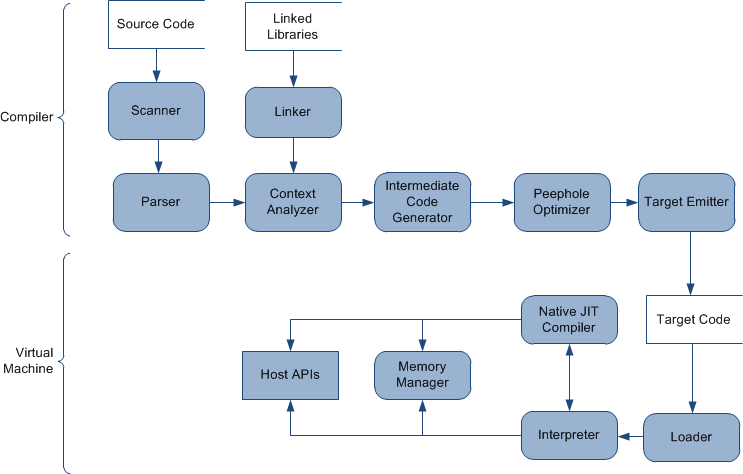
\includegraphics[scale=0.60]{../images/compiler_data_flow.png}

The following section gives a brief overview of the major architectural components the comprise the Objeck language compiler and virtual machine.

\subsection{Compiler}
The language compiler is written in C++ and makes heavy use of the C++ STL for portability across platforms.  As mentioned in the introduction, the compiler accepts source files and shared libraries as inputs and produces either executables or shared libraries.  Note, the compiler has two modes of operation: \texttt{User Mode} compiles traditional end-user programs, while \texttt{System Mode} compiles system libraries and processes special system language directives.

\subsubsection{Scanner and Parser}
The scanner component reads source files and parses the text into tokens.  The scanner works in conjugation with the \emph{LL(k)} parser by providing \emph{k} lookahead tokens for parsing.  Note, the scanner can only scan system language directives while in \texttt{System Mode}.  The source parser is a recursive-decent parser that generates an abstract parser tree, which is passed to the Contextual Analyser for validation.

\subsubsection{Contextual Analyser}
The Contextual Analyser is responsible for ensuring that a source program is valid.  In addition, the context analyser also creates relationships between contextually resolved entities (i.e. methods $\longleftrightarrow$ method calls).  The analyser accepts an abstract parser tree and shared libraries as input and produces a decorated parse tree as output.  The decorated parse tree is then passed to the Intermediate Code Generator for the production of VM instructions.

\subsubsection{Intermediate Code Generator and Optimzier}
The Intermediate Code Generator accpets a decorated parse and produces a flat list of VM stack instructions.  These instruction lists are then passed to the Optimizer for basic block optimizations (constant folding, strength reduction, instruction simplification and method inlining).

\subsubsection{Target Emitter}
Finally, the improved intermediate code is passed to code emitter component, which writes it to a file.

\subsection{Virtual Machine}
The language VM is written in C/C++ and was designed to be highly portable.  The VM makes heavy use of operating system specific APIs (i.e. WIN32 and POSIX) but does so in an abstracted manner.  The JIT compiler is targeted to produce machine code for the IA-32 and AMD64 (future) hardware architectures.  

\subsubsection{Loader}
The loader component allows the VM to read target code structures such as classes, methods and VM instructions.  The loader create an in-memory representation of this information, which is used by the VM interpreter and JIT compiler.  In addition, the loader processes command-line parameters that are passed into the VM prior to execution.

\subsubsection{Interpreter}
The Interpreter executes stack based VM instructions (listed below) and manages two primary stacks: the execution stack and call stack.  The execution stack is used to manage the data that is needed for VM calculations.  The call stack is used to manage function/method calls and the states between those calls.

\subsubsection{JIT Compiler}
The JIT compiler translates stack based VM instruction into processor specific machine code (i.e. IA-32).  The JIT compiler is evoked by the interpreter and methods are translated in a separate execution thread.  This process allow methods to be executed concurrently in an interpreted manner while they are being compiled into machine code.  Note, methods are only converted into machine code once.

\subsubsection{Memory Manager}
The Memory Manager component allows the runtime system to manage the user allocation/deallocation of heap memory.  The memory mangers implementes a multi-thread ``mark and sweep'' algorithm.  The marking stage of the process is multi-thread, such that, each root in scanned in a separate thread.  The sweeping stage is done in a single thread since the data structures that are needed to manage the state of the running program are modified.

\section{Appendix B: VM Instructions}
The appendix below lists the types of stack instructions that are executed by the Objeck VM.  The VM was designed to be portable and language independent.  Early development versions of the VM included an inline assembler, which may be re-added in future releases.

\begin{center}
{\small{
\begin{tabular}{| l | l | p{6 cm} |}
\hline
\multicolumn{3}{|c|}{\textbf{Stack Operators}} \\
\hline
\emph{Mnemonic}  &  \emph{Opcode(s)}  &  \emph{Description} \\ \hline \hline
LOAD\_INT\_LIT & 4-byte integer & pushes integer onto stack  \\ \hline
LOAD\_FLOAT\_LIT & 8-byte float & pushes float onto stack \\ \hline
LOAD\_INT\_VAR & variable index & pushes integer onto stack \\ \hline
LOAD\_FLOAT\_VAR & variable index & pushes float onto stack \\ \hline
LOAD\_SELF & n/a & pushes self integer on stack \\ \hline
STOR\_INT\_VAR & variable index & pops integer from stack and saves to index location \\ \hline
STOR\_FLOAT\_VAR & variable index & pops float from stack and saves to index location \\ \hline
COPY\_INT\_VAR & variable index & copies an integer from stack and saves to index location \\ \hline
COPY\_FLOAT\_VAR & variable index & copies a float from stack and saves to index location \\ \hline
LOAD\_BYTE\_ARY\_ELM & array dimension & pushes byte onto stack; assumes array address was pushed prior \\ \hline
LOAD\_INT\_ARY\_ELM & array dimension & pushes integer onto stack; assumes array address was pushed prior \\ \hline
LOAD\_FLOAT\_ARY\_ELM & array dimension & pushes float onto stack; assumes array address was pushed prior \\ \hline
LOAD\_ARY\_SIZE & n/a & pushes array size as integer onto stack; assumes array address was pushed prior \\ \hline
STOR\_BYTE\_ARY\_ELM & variable index & stores byte at index location; assumes array address was pushed prior \\ \hline
STOR\_INT\_ARY\_ELM & variable index & stores integer at index location ; assumes array address was pushed prior \\ \hline
STOR\_FLOAT\_ARY\_ELM & variable index & stores float at index location; assumes array address was pushed prior \\ \hline
\end{tabular}

\vspace{\baselineskip}
\begin{tabular}{| l | l | p{6 cm} |}
\hline
\multicolumn{3}{|c|}{\textbf{Logical Operators}} \\
\hline
\emph{Mnemonic}  &  \emph{Opcode(s)}  &  \emph{Description} \\ \hline \hline
EQL\_INT & n/a & pops top two integer values and pushes result of equal operation \\ \hline
NEQL\_INT & n/a & pops top two integer values and pushes result of not-equal operation \\ \hline
LES\_INT & n/a & pops top two integer values and pushes result of less-than operation \\ \hline
GTR\_INT & n/a & pops top two integer values and pushes result of greater-than operation \\ \hline
LES\_EQL\_INT & n/a & pops top two integer values and pushes result of less-than-equal operation \\ \hline
GTR\_EQL\_INT & n/a & pops top two integer values and pushes result of greater-than-equal operation \\ \hline
EQL\_FLOAT & n/a & pops top two floats values and pushes result of equal operation \\ \hline
NEQL\_FLOAT & n/a & pops top two floats values and pushes result of not-equal operation \\ \hline
LES\_FLOAT & n/a & pops top two floats values and pushes result of less-than operation \\ \hline
GTR\_FLOAT & n/a & pops top two floats values and pushes result of greater-than operation \\ \hline
LES\_EQL\_FLOAT & n/a & pops top two floats values and pushes result of less-than-equal operation \\ \hline
GTR\_EQL\_FLOAT & n/a & pops top two floats values and pushes result of greater-than-equal operation \\ \hline
AND\_INT & n/a & pops top two integer values and pushes result of add operation \\ \hline
OR\_INT & n/a & pops top two integer values and pushes result of or operation \\ \hline
\end{tabular}

\vspace{\baselineskip}
\begin{tabular}{| l | l | p{6 cm} |}
\hline
\multicolumn{3}{|c|}{\textbf{Mathematical Operators}} \\
\hline
\emph{Mnemonic}  &  \emph{Opcode(s)}  &  \emph{Description} \\ \hline \hline
ADD\_INT & n/a & pops top two integer values and pushes result of add operation \\ \hline
SUB\_INT & n/a & pops top two integer values and pushes result of subtract operation \\ \hline
MUL\_INT & n/a & pops top two integer values and pushes result of multiply operation \\ \hline
DIV\_INT & n/a & pops top two integer values and pushes result of divide operation \\ \hline
SHL\_INT & n/a & pops top two floats values and pushes result of shift left operation \\ \hline
SHR\_INT & n/a & pops top two floats values and pushes result of shift right operation \\ \hline
MOD\_INT & n/a & pops top two integer values and pushes result of modulus operation \\ \hline
ADD\_FLOAT & n/a & pops top two floats values and pushes result of greater-than-equal operation \\ \hline
SUB\_FLOAT & n/a & pops top two floats values and pushes result of subtract operation \\ \hline
MUL\_FLOAT & n/a & pops top two floats values and pushes result of multiply operation \\ \hline
DIV\_FLOAT & n/a & pops top two floats values and pushes result of divide operation \\ \hline
I2F & n/a & pop top integer and pushes result of float cast \\ \hline
F2I & n/a & pop top float and pushes result of integer cast \\ \hline
\end{tabular}

\vspace{\baselineskip}
\begin{tabular}{| l | p{4 cm} | p{6 cm} |}
\hline
\multicolumn{3}{|c|}{\textbf{Objects/Methods/Traps}} \\
\hline
\emph{Mnemonic}  &  \emph{Opcode(s)}  &  \emph{Description} \\ \hline \hline
SWAP\_INT & n/a & swaps the top two integer values on the stack \\ \hline
POP\_INT & n/a & control pop of an integer from the stack \\ \hline
POP\_FLOAT & n/a & control pop of a float from the stack \\ \hline
RTRN & n/a & exits existing method returning control to callee \\ \hline
MTHD\_CALL & integer values for class id and method id & synchronous call to given method releasing control \\ \hline
ASYNC\_MTHD\_CALL & integer values for class id and method id; pushes new thread id & asynchronous call to given method \\ \hline
ASYNC\_JOIN & thread id & waits for identified thread to end execution \\ \hline
LBL & label id & identifies a jump label \\ \hline
JMP & label id and conditional context (1=true, 0=unconditional, -1=false) & jump to label id \\ \hline
NEW\_BYTE\_ARY & array dimension & pushes address of new byte array \\ \hline
NEW\_INT\_ARY & array dimension & pushes address of new integer array \\ \hline
NEW\_FLOAT\_ARY & array dimension & pushes address of new float array \\ \hline
NEW\_OBJ\_INST & integer value for class id & pushes address of new class instance \\ \hline
OBJ\_INST\_CAST & integer values for ``from'' class and ``to'' class & performs runtime class cast check (note: only required for up casting) \\ \hline
THREAD\_CREATE & n/a & creates an new thread instance (calculation stack and  stack pointer) \\ \hline
THREAD\_WAIT & n/a & waits for worker threads to stop execution \\ \hline
CRITICAL\_START & n/a & creates a mutex such that only one thread can execute in a given section \\ \hline
CRITICAL\_END & n/a & releases a system mutex \\ \hline
TRAP & integer value for trap id & calls runtime subroutine releasing control \\ \hline
TRAP\_RTRN & integer value for trap id and number of arguments & calls runtime subroutine releasing control and then process an integer return value \\ \hline
LIB\_NEW\_OBJ\_INST & n/a & symbolic library link for a new object instance  \\ \hline
LIB\_MTHD\_CALL & n/a & symbolic library link for a method call  \\ \hline
LIB\_OBJ\_INST\_CAST & n/a & symbolic library link for an object cast  \\ \hline
\end{tabular}
}}
\end{center}

\end{document}
